\documentclass{article}
\usepackage{graphicx}
\usepackage[absolute,overlay]{textpos}
\setlength{\parindent}{0pt}
\usepackage{geometry}
\geometry{top=1in, bottom=1in, right=1in, left=1in}
\usepackage{multicol}
\usepackage{multirow}
\usepackage[pages=some]{background}

\usepackage{listings}
\usepackage{xcolor}

\pagestyle{empty}

\backgroundsetup{
  scale=1,
  opacity=1,
  angle=0,
  contents={
\includegraphics[width=\paperwidth,height=\paperheight]{portada.jpg}}
}

\definecolor{rojo}{rgb}{0.8, 0, 0}

\usepackage{titlesec}

\titleformat{\section}
  {\color{rojo}\Large\bfseries}
  {}
  {0pt}
  {}

\titleformat{\subsection}
  {\color{rojo}\large\bfseries}
  {}
  {0pt}
  {}

\begin{document}

\BgThispage
\-
\begin{textblock*}{15cm}(4cm, 9cm)
    {\fontsize{30pt}{16pt}\selectfont
    \textcolor{rojo}{\textbf{REPORTE DE PRÁCTICA NO. 7}}
    }
\end{textblock*}

\begin{textblock*}{15cm}(3cm, 11cm)
    {\fontsize{15pt}{16pt}\selectfont
    \centering
    \textcolor{rojo}{\textbf{ANÁLISIS SINTÁCTICO DE ELEMENTOS DE UN LENGUAJE DE PROGRAMACIÓN}}
    }
\end{textblock*}

\begin{textblock*}{15cm}(4cm, 13cm)
    {\fontsize{13pt}{16pt}\selectfont
    \textcolor{rojo}{\textbf{ALUMNOS: \\ Raúl Arana Juárez \\
    Colmenares Garcia Andres\\
    Flores Oliver Alain
    }}
    }
\end{textblock*}

\begin{textblock*}{15cm}(4cm, 15cm)
    {\fontsize{11pt}{16pt}\selectfont
    \textcolor{rojo}{\textbf{Dr. Eduardo Cornejo-Velázquez}}
    }
\end{textblock*}

\newpage

\section{1. Introducción}

El análisis sintáctico en lenguajes basados en gramáticas formales resulta esencial para facilitar la 
comprensión del compilador y abordar de manera más efectiva errores difíciles de identificar, como la 
ambigüedad en el reconocimiento de ciertas sentencias. El analizador sintáctico opera sobre una gramática 
de contexto libre, que establece las reglas para la formación de las estructuras del lenguaje. 

Gramática de contexto libre:  

G (N, T, P, S) 

N = No terminales.  
T = Terminales.  
P = Reglas de Producción.  
S = Axioma Inicial.  

Ejemplo: Se considera la gramática que reconoce las operaciones aritméticas.  

E → E + T  
| T  

T → T * F  
| F  

F → ID  
| NUM  
| (E)  

En el que:  
N = \{E, T, F\}  
T = \{ID, NUM, (, ), +, *\}  
P = Reglas de producción  
S = E  

\section{2. Marco teórico}

El análisis sintáctico es una fase del proceso de compilación que se encarga de verificar que una secuencia de tokens cumple con una gramática definida. Para ello se utilizan gramáticas de contexto libre, las cuales permiten modelar estructuras complejas como expresiones y sentencias condicionales.

Las herramientas Lex y Yacc permiten automatizar este proceso:
\begin{itemize}
\item Lex: Genera el analizador léxico.
\item Yacc: Genera el analizador sintáctico.
\end{itemize}

Además, conceptos como derivación por la izquierda y por la derecha son fundamentales para construir árboles sintácticos.


\subsection{3. Objetivo General}

Implementar un analizador léxico y un analizador sintáctico utilizando Lex y Yacc para reconocer y validar 
la estructura condicional if - then capaz de realizar la detección de errores y la validación de gramáticas 
en un lenguaje de programación de alto nivel.

\subsection{Objetivos Específicos}

\begin{itemize}
\item Emplear las herramientas conceptuales (autómatas y gramáticas libres de contexto) para definir cómo lograr el objetivo de la práctica.
\item Diseñar un programa en Lex que identifique los tokens asociados a las palabras clave if, then, expresiones condicionales y bloques de código.
\item Implementar un programa en Yacc que verifique la correcta construcción de la estructura if...then mediante una gramática formal.
\end{itemize}

\section{4. Desarrollo}

\subsection{Código en Yacc}

\begin{lstlisting}[language=C]
%{
#include <stdio.h>
int yylex();
int yyerror(const char *s) {
    printf("Expresion NO valida\n");
    return 0;
}
%}

%token ENTERO DECIMAL SIMBOLO COMPARACION ID EOL CONDIF CONDELSE
%left SIMBOLO
%left COMPARACION
%left CONDIF
%start input

%%

input:
      input cond EOL { printf("Expresion valida\n"); }
    | /* vacío */
;

expr:
      expr SIMBOLO expr
    | expr COMPARACION expr
    | '(' expr ')'
    | ENTERO
    | DECIMAL
    | ID
;

cond: 
      CONDIF '(' expr ')' '{' '}'
    | CONDIF '(' expr ')' '{' '}' CONDELSE '{' '}'
;
%%
\end{lstlisting}

\subsection{Archivo de Entrada}

\begin{figure}[h]
\centering
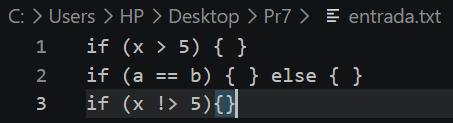
\includegraphics[width=0.8\textwidth]{entrada.png}
\caption{Valores de entrada 1}
\end{figure}

\begin{figure}[h]
\centering
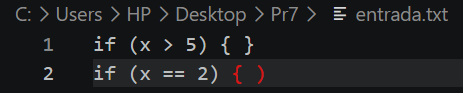
\includegraphics[width=0.8\textwidth]{entrada2.png}
\caption{Valores de entrada 2}
\end{figure}


\subsection{Ejecución}

Se ejecutaron los siguientes comandos desde el CMD:

\begin{verbatim}
flex archivo.l
yacc -d parser.y
gcc lex.yy.c parser.tab.c -o main
./main.exe
\end{verbatim}


\section{Resultados}

El programa produjo la siguiente salida:

\begin{figure}[h]
\centering
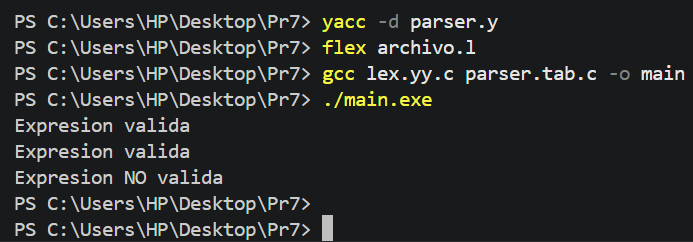
\includegraphics[width=0.8\textwidth]{resultado_valido.png}
\caption{Resultado con expresiones 1}
\end{figure}

\begin{figure}[h]
\centering
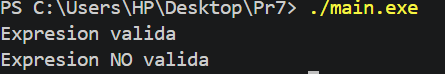
\includegraphics[width=0.8\textwidth]{resultado_valido2.png}
\caption{Resultado con expresiones 2}
\end{figure}

Esto demuestra que ambas estructuras condicionales fueron reconocidas de manera correcta por el analizador sintáctico.

\section{Cuestionario}

\textbf{1. ¿Cuáles son las principales ventajas de usar gramáticas de contexto libre?}

Permiten definir de manera clara y estructurada la sintaxis de un lenguaje, facilitando la detección de errores. Además, son suficientemente expresivas para representar estructuras como expresiones y condicionales, y son compatibles con herramientas como Yacc.

\textbf{2. ¿Qué tipo de errores fueron detectados?}

Errores sintácticos como:
\begin{itemize}
\item Falta de paréntesis
\item Uso incorrecto de operadores
\item Estructuras if mal formadas
\end{itemize}
Las gramáticas permiten identificar estos errores al no cumplir con las reglas definidas.

\textbf{3. ¿Cómo contribuyen las derivaciones?}

Permiten construir el árbol sintáctico paso a paso. La derivación por la izquierda y por la derecha ayudan a determinar el orden en que se expanden los símbolos, lo cual es fundamental para validar la estructura de manera correcta.

\textbf{4. ¿Qué ajustes se necesitan para if...then...else?}

Se debe ampliar la gramática agregando reglas que incluyan la parte else:
\begin{verbatim}
CONDIF '(' expr ')' '{' '}' CONDELSE '{' '}'
\end{verbatim}

\section{Conclusiones}

Se logró implementar correctamente un analizador sintáctico utilizando Lex y Yacc, donde el sistema es capaz de validar estructuras condicionales y detectar errores sintácticos.

Esta práctica nos permitió comprender mejor el funcionamiento de los compiladores y la importancia de las gramáticas de contexto libre en la validación de lenguajes de programación.

\section{Bibliografía}

Aho, A. V., Ravi, S. A. V., Ullman, J. D. (1998). Compiladores: Principios, técnicas y herramientas.

Giró, J., Vázquez, J., Meloni, B., Constable, L. (2015). Lenguajes formales y teoría de autómatas.

\end{document}